% Options for packages loaded elsewhere
\PassOptionsToPackage{unicode}{hyperref}
\PassOptionsToPackage{hyphens}{url}
%
\documentclass[
]{article}
\usepackage{amsmath,amssymb}
\usepackage{iftex}
\ifPDFTeX
  \usepackage[T1]{fontenc}
  \usepackage[utf8]{inputenc}
  \usepackage{textcomp} % provide euro and other symbols
\else % if luatex or xetex
  \usepackage{unicode-math} % this also loads fontspec
  \defaultfontfeatures{Scale=MatchLowercase}
  \defaultfontfeatures[\rmfamily]{Ligatures=TeX,Scale=1}
\fi
\usepackage{lmodern}
\ifPDFTeX\else
  % xetex/luatex font selection
\fi
% Use upquote if available, for straight quotes in verbatim environments
\IfFileExists{upquote.sty}{\usepackage{upquote}}{}
\IfFileExists{microtype.sty}{% use microtype if available
  \usepackage[]{microtype}
  \UseMicrotypeSet[protrusion]{basicmath} % disable protrusion for tt fonts
}{}
\makeatletter
\@ifundefined{KOMAClassName}{% if non-KOMA class
  \IfFileExists{parskip.sty}{%
    \usepackage{parskip}
  }{% else
    \setlength{\parindent}{0pt}
    \setlength{\parskip}{6pt plus 2pt minus 1pt}}
}{% if KOMA class
  \KOMAoptions{parskip=half}}
\makeatother
\usepackage{xcolor}
\usepackage[margin=1in]{geometry}
\usepackage{color}
\usepackage{fancyvrb}
\newcommand{\VerbBar}{|}
\newcommand{\VERB}{\Verb[commandchars=\\\{\}]}
\DefineVerbatimEnvironment{Highlighting}{Verbatim}{commandchars=\\\{\}}
% Add ',fontsize=\small' for more characters per line
\usepackage{framed}
\definecolor{shadecolor}{RGB}{248,248,248}
\newenvironment{Shaded}{\begin{snugshade}}{\end{snugshade}}
\newcommand{\AlertTok}[1]{\textcolor[rgb]{0.94,0.16,0.16}{#1}}
\newcommand{\AnnotationTok}[1]{\textcolor[rgb]{0.56,0.35,0.01}{\textbf{\textit{#1}}}}
\newcommand{\AttributeTok}[1]{\textcolor[rgb]{0.13,0.29,0.53}{#1}}
\newcommand{\BaseNTok}[1]{\textcolor[rgb]{0.00,0.00,0.81}{#1}}
\newcommand{\BuiltInTok}[1]{#1}
\newcommand{\CharTok}[1]{\textcolor[rgb]{0.31,0.60,0.02}{#1}}
\newcommand{\CommentTok}[1]{\textcolor[rgb]{0.56,0.35,0.01}{\textit{#1}}}
\newcommand{\CommentVarTok}[1]{\textcolor[rgb]{0.56,0.35,0.01}{\textbf{\textit{#1}}}}
\newcommand{\ConstantTok}[1]{\textcolor[rgb]{0.56,0.35,0.01}{#1}}
\newcommand{\ControlFlowTok}[1]{\textcolor[rgb]{0.13,0.29,0.53}{\textbf{#1}}}
\newcommand{\DataTypeTok}[1]{\textcolor[rgb]{0.13,0.29,0.53}{#1}}
\newcommand{\DecValTok}[1]{\textcolor[rgb]{0.00,0.00,0.81}{#1}}
\newcommand{\DocumentationTok}[1]{\textcolor[rgb]{0.56,0.35,0.01}{\textbf{\textit{#1}}}}
\newcommand{\ErrorTok}[1]{\textcolor[rgb]{0.64,0.00,0.00}{\textbf{#1}}}
\newcommand{\ExtensionTok}[1]{#1}
\newcommand{\FloatTok}[1]{\textcolor[rgb]{0.00,0.00,0.81}{#1}}
\newcommand{\FunctionTok}[1]{\textcolor[rgb]{0.13,0.29,0.53}{\textbf{#1}}}
\newcommand{\ImportTok}[1]{#1}
\newcommand{\InformationTok}[1]{\textcolor[rgb]{0.56,0.35,0.01}{\textbf{\textit{#1}}}}
\newcommand{\KeywordTok}[1]{\textcolor[rgb]{0.13,0.29,0.53}{\textbf{#1}}}
\newcommand{\NormalTok}[1]{#1}
\newcommand{\OperatorTok}[1]{\textcolor[rgb]{0.81,0.36,0.00}{\textbf{#1}}}
\newcommand{\OtherTok}[1]{\textcolor[rgb]{0.56,0.35,0.01}{#1}}
\newcommand{\PreprocessorTok}[1]{\textcolor[rgb]{0.56,0.35,0.01}{\textit{#1}}}
\newcommand{\RegionMarkerTok}[1]{#1}
\newcommand{\SpecialCharTok}[1]{\textcolor[rgb]{0.81,0.36,0.00}{\textbf{#1}}}
\newcommand{\SpecialStringTok}[1]{\textcolor[rgb]{0.31,0.60,0.02}{#1}}
\newcommand{\StringTok}[1]{\textcolor[rgb]{0.31,0.60,0.02}{#1}}
\newcommand{\VariableTok}[1]{\textcolor[rgb]{0.00,0.00,0.00}{#1}}
\newcommand{\VerbatimStringTok}[1]{\textcolor[rgb]{0.31,0.60,0.02}{#1}}
\newcommand{\WarningTok}[1]{\textcolor[rgb]{0.56,0.35,0.01}{\textbf{\textit{#1}}}}
\usepackage{graphicx}
\makeatletter
\def\maxwidth{\ifdim\Gin@nat@width>\linewidth\linewidth\else\Gin@nat@width\fi}
\def\maxheight{\ifdim\Gin@nat@height>\textheight\textheight\else\Gin@nat@height\fi}
\makeatother
% Scale images if necessary, so that they will not overflow the page
% margins by default, and it is still possible to overwrite the defaults
% using explicit options in \includegraphics[width, height, ...]{}
\setkeys{Gin}{width=\maxwidth,height=\maxheight,keepaspectratio}
% Set default figure placement to htbp
\makeatletter
\def\fps@figure{htbp}
\makeatother
\setlength{\emergencystretch}{3em} % prevent overfull lines
\providecommand{\tightlist}{%
  \setlength{\itemsep}{0pt}\setlength{\parskip}{0pt}}
\setcounter{secnumdepth}{-\maxdimen} % remove section numbering
\usepackage{booktabs}
\usepackage{longtable}
\usepackage{array}
\usepackage{multirow}
\usepackage{wrapfig}
\usepackage{float}
\usepackage{colortbl}
\usepackage{pdflscape}
\usepackage{tabu}
\usepackage{threeparttable}
\usepackage{threeparttablex}
\usepackage[normalem]{ulem}
\usepackage{makecell}
\usepackage{xcolor}
\ifLuaTeX
  \usepackage{selnolig}  % disable illegal ligatures
\fi
\IfFileExists{bookmark.sty}{\usepackage{bookmark}}{\usepackage{hyperref}}
\IfFileExists{xurl.sty}{\usepackage{xurl}}{} % add URL line breaks if available
\urlstyle{same}
\hypersetup{
  pdftitle={Proyecto 1},
  pdfauthor={Camilo Rojas},
  hidelinks,
  pdfcreator={LaTeX via pandoc}}

\title{Proyecto 1}
\author{Camilo Rojas}
\date{2023-10-11}

\begin{document}
\maketitle

\begin{Shaded}
\begin{Highlighting}[]
\CommentTok{\#tinytex::install\_tinytex()}
\FunctionTok{library}\NormalTok{(latexpdf)}
\FunctionTok{library}\NormalTok{(knitr)}
\NormalTok{opts\_chunk}\SpecialCharTok{$}\FunctionTok{set}\NormalTok{(}\AttributeTok{echo =} \ConstantTok{TRUE}\NormalTok{)}
\end{Highlighting}
\end{Shaded}

\hypertarget{first-question}{%
\section{First question}\label{first-question}}

I load the dataset and named it as \textbf{\emph{data}}

\begin{Shaded}
\begin{Highlighting}[]
\FunctionTok{library}\NormalTok{(rio)}

\NormalTok{data }\OtherTok{\textless{}{-}} \FunctionTok{import}\NormalTok{(}\StringTok{"./activity.csv"}\NormalTok{)}

\NormalTok{data}\SpecialCharTok{$}\NormalTok{steps }\OtherTok{\textless{}{-}} \FunctionTok{as.numeric}\NormalTok{(data}\SpecialCharTok{$}\NormalTok{steps)}
\NormalTok{data}\SpecialCharTok{$}\NormalTok{date }\OtherTok{\textless{}{-}} \FunctionTok{as.Date}\NormalTok{(data}\SpecialCharTok{$}\NormalTok{date)}
\end{Highlighting}
\end{Shaded}

\hypertarget{second-question}{%
\section{second question}\label{second-question}}

\begin{Shaded}
\begin{Highlighting}[]
\NormalTok{total\_steps }\OtherTok{\textless{}{-}} \FunctionTok{sum}\NormalTok{(data}\SpecialCharTok{$}\NormalTok{steps, }\AttributeTok{na.rm =}\NormalTok{ T)}
\end{Highlighting}
\end{Shaded}

\begin{enumerate}
\def\labelenumi{\arabic{enumi}.}
\item
  the number total of steps in this dataset is
  \ensuremath{5.70608\times 10^{5}}
\item
  i did the histogram per day vs number of steps
\end{enumerate}

\begin{Shaded}
\begin{Highlighting}[]
\FunctionTok{library}\NormalTok{(dplyr)}
\end{Highlighting}
\end{Shaded}

\begin{verbatim}
## 
## Attaching package: 'dplyr'
\end{verbatim}

\begin{verbatim}
## The following objects are masked from 'package:stats':
## 
##     filter, lag
\end{verbatim}

\begin{verbatim}
## The following objects are masked from 'package:base':
## 
##     intersect, setdiff, setequal, union
\end{verbatim}

\begin{Shaded}
\begin{Highlighting}[]
\FunctionTok{library}\NormalTok{(ggplot2)}

\NormalTok{data }\SpecialCharTok{\%\textgreater{}\%}
 \FunctionTok{filter}\NormalTok{(}\SpecialCharTok{!}\FunctionTok{is.na}\NormalTok{(steps)) }\SpecialCharTok{\%\textgreater{}\%}
 \FunctionTok{ggplot}\NormalTok{() }\SpecialCharTok{+}
  \FunctionTok{aes}\NormalTok{(}\AttributeTok{x =}\NormalTok{ date, }\AttributeTok{weight =}\NormalTok{ steps) }\SpecialCharTok{+}
  \FunctionTok{geom\_bar}\NormalTok{(}\AttributeTok{fill =} \StringTok{"\#112446"}\NormalTok{) }\SpecialCharTok{+}
  \FunctionTok{labs}\NormalTok{(}
    \AttributeTok{x =} \StringTok{"Day"}\NormalTok{,}
    \AttributeTok{y =} \StringTok{"number of steps"}\NormalTok{,}
    \AttributeTok{title =} \StringTok{"steps per day"}
\NormalTok{  ) }\SpecialCharTok{+}
  \FunctionTok{theme\_classic}\NormalTok{()}
\end{Highlighting}
\end{Shaded}

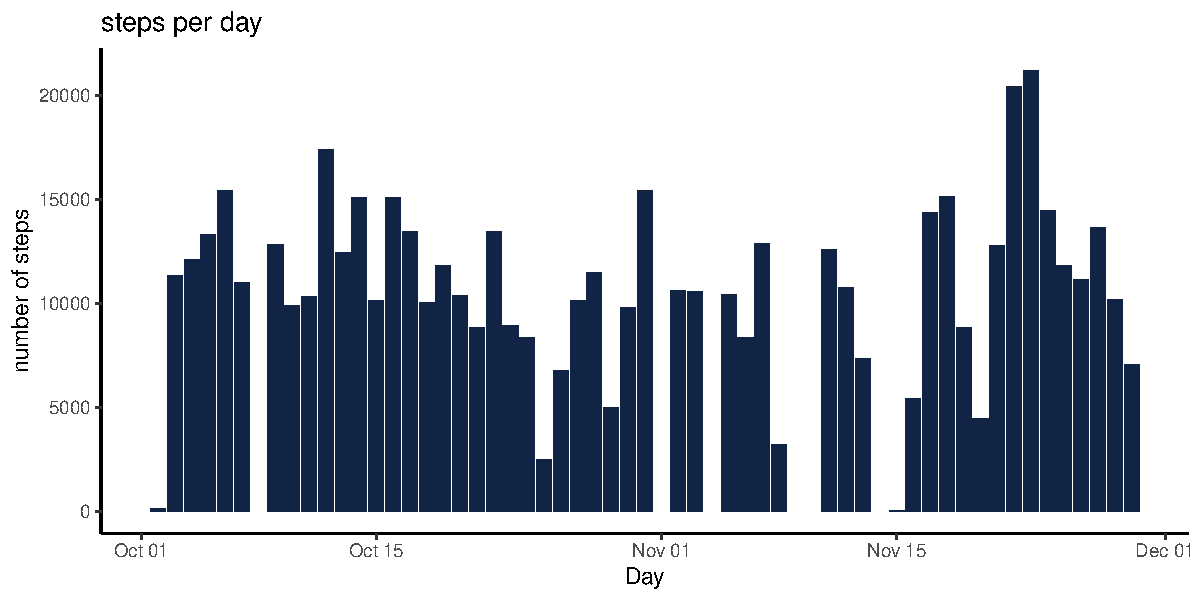
\includegraphics{project1_files/figure-latex/unnamed-chunk-4-1.pdf} 3.
the next table show report the mean and median of the total number of
steps taken per day

\begin{Shaded}
\begin{Highlighting}[]
\FunctionTok{library}\NormalTok{(kableExtra)}
\end{Highlighting}
\end{Shaded}

\begin{verbatim}
## 
## Attaching package: 'kableExtra'
\end{verbatim}

\begin{verbatim}
## The following object is masked from 'package:dplyr':
## 
##     group_rows
\end{verbatim}

\begin{Shaded}
\begin{Highlighting}[]
\FunctionTok{library}\NormalTok{(dplyr)}
\NormalTok{data1 }\OtherTok{\textless{}{-}}\NormalTok{ data }\SpecialCharTok{\%\textgreater{}\%} 
        \FunctionTok{select}\NormalTok{(date, steps) }\SpecialCharTok{\%\textgreater{}\%} 
        \FunctionTok{group\_by}\NormalTok{(date) }\SpecialCharTok{\%\textgreater{}\%} 
        \FunctionTok{summarise}\NormalTok{(}\AttributeTok{median =} \FunctionTok{median}\NormalTok{(steps,}\AttributeTok{na.rm =}\NormalTok{ T), }\AttributeTok{mean =} \FunctionTok{mean}\NormalTok{(steps,}\AttributeTok{na.rm =}\NormalTok{ T))}
\NormalTok{data1}\SpecialCharTok{$}\NormalTok{mean }\OtherTok{\textless{}{-}} \FunctionTok{ifelse}\NormalTok{(}\FunctionTok{is.nan}\NormalTok{(data1}\SpecialCharTok{$}\NormalTok{mean),}\DecValTok{0}\NormalTok{,data1}\SpecialCharTok{$}\NormalTok{mean)}
\NormalTok{data1}\SpecialCharTok{$}\NormalTok{median }\OtherTok{\textless{}{-}} \FunctionTok{ifelse}\NormalTok{(}\FunctionTok{is.nan}\NormalTok{(data1}\SpecialCharTok{$}\NormalTok{median),}\DecValTok{0}\NormalTok{,data1}\SpecialCharTok{$}\NormalTok{median)}
\FunctionTok{kbl}\NormalTok{(data1) }\SpecialCharTok{\%\textgreater{}\%} 
        \FunctionTok{kable\_styling}\NormalTok{()}
\end{Highlighting}
\end{Shaded}

\begin{table}
\centering
\begin{tabular}[t]{l|r|r}
\hline
date & median & mean\\
\hline
2012-10-01 & NA & 0.0000000\\
\hline
2012-10-02 & 0 & 0.4375000\\
\hline
2012-10-03 & 0 & 39.4166667\\
\hline
2012-10-04 & 0 & 42.0694444\\
\hline
2012-10-05 & 0 & 46.1597222\\
\hline
2012-10-06 & 0 & 53.5416667\\
\hline
2012-10-07 & 0 & 38.2465278\\
\hline
2012-10-08 & NA & 0.0000000\\
\hline
2012-10-09 & 0 & 44.4826389\\
\hline
2012-10-10 & 0 & 34.3750000\\
\hline
2012-10-11 & 0 & 35.7777778\\
\hline
2012-10-12 & 0 & 60.3541667\\
\hline
2012-10-13 & 0 & 43.1458333\\
\hline
2012-10-14 & 0 & 52.4236111\\
\hline
2012-10-15 & 0 & 35.2048611\\
\hline
2012-10-16 & 0 & 52.3750000\\
\hline
2012-10-17 & 0 & 46.7083333\\
\hline
2012-10-18 & 0 & 34.9166667\\
\hline
2012-10-19 & 0 & 41.0729167\\
\hline
2012-10-20 & 0 & 36.0937500\\
\hline
2012-10-21 & 0 & 30.6284722\\
\hline
2012-10-22 & 0 & 46.7361111\\
\hline
2012-10-23 & 0 & 30.9652778\\
\hline
2012-10-24 & 0 & 29.0104167\\
\hline
2012-10-25 & 0 & 8.6527778\\
\hline
2012-10-26 & 0 & 23.5347222\\
\hline
2012-10-27 & 0 & 35.1354167\\
\hline
2012-10-28 & 0 & 39.7847222\\
\hline
2012-10-29 & 0 & 17.4236111\\
\hline
2012-10-30 & 0 & 34.0937500\\
\hline
2012-10-31 & 0 & 53.5208333\\
\hline
2012-11-01 & NA & 0.0000000\\
\hline
2012-11-02 & 0 & 36.8055556\\
\hline
2012-11-03 & 0 & 36.7048611\\
\hline
2012-11-04 & NA & 0.0000000\\
\hline
2012-11-05 & 0 & 36.2465278\\
\hline
2012-11-06 & 0 & 28.9375000\\
\hline
2012-11-07 & 0 & 44.7326389\\
\hline
2012-11-08 & 0 & 11.1770833\\
\hline
2012-11-09 & NA & 0.0000000\\
\hline
2012-11-10 & NA & 0.0000000\\
\hline
2012-11-11 & 0 & 43.7777778\\
\hline
2012-11-12 & 0 & 37.3784722\\
\hline
2012-11-13 & 0 & 25.4722222\\
\hline
2012-11-14 & NA & 0.0000000\\
\hline
2012-11-15 & 0 & 0.1423611\\
\hline
2012-11-16 & 0 & 18.8923611\\
\hline
2012-11-17 & 0 & 49.7881944\\
\hline
2012-11-18 & 0 & 52.4652778\\
\hline
2012-11-19 & 0 & 30.6979167\\
\hline
2012-11-20 & 0 & 15.5277778\\
\hline
2012-11-21 & 0 & 44.3993056\\
\hline
2012-11-22 & 0 & 70.9270833\\
\hline
2012-11-23 & 0 & 73.5902778\\
\hline
2012-11-24 & 0 & 50.2708333\\
\hline
2012-11-25 & 0 & 41.0902778\\
\hline
2012-11-26 & 0 & 38.7569444\\
\hline
2012-11-27 & 0 & 47.3819444\\
\hline
2012-11-28 & 0 & 35.3576389\\
\hline
2012-11-29 & 0 & 24.4687500\\
\hline
2012-11-30 & NA & 0.0000000\\
\hline
\end{tabular}
\end{table}

\hypertarget{third-question}{%
\section{third question}\label{third-question}}

time series plot for 5-minute interval

\begin{Shaded}
\begin{Highlighting}[]
\NormalTok{interval5 }\OtherTok{\textless{}{-}}\NormalTok{ data }\SpecialCharTok{\%\textgreater{}\%} 
        \FunctionTok{filter}\NormalTok{(interval }\SpecialCharTok{==} \DecValTok{5}\NormalTok{)}

\NormalTok{interval5 }\SpecialCharTok{\%\textgreater{}\%}
 \FunctionTok{filter}\NormalTok{(}\SpecialCharTok{!}\FunctionTok{is.na}\NormalTok{(steps)) }\SpecialCharTok{\%\textgreater{}\%}
 \FunctionTok{ggplot}\NormalTok{() }\SpecialCharTok{+}
  \FunctionTok{aes}\NormalTok{(}\AttributeTok{x =}\NormalTok{ date, }\AttributeTok{weight =}\NormalTok{ steps) }\SpecialCharTok{+}
  \FunctionTok{geom\_bar}\NormalTok{(}\AttributeTok{fill =} \StringTok{"\#112446"}\NormalTok{) }\SpecialCharTok{+}
  \FunctionTok{theme\_minimal}\NormalTok{()}
\end{Highlighting}
\end{Shaded}

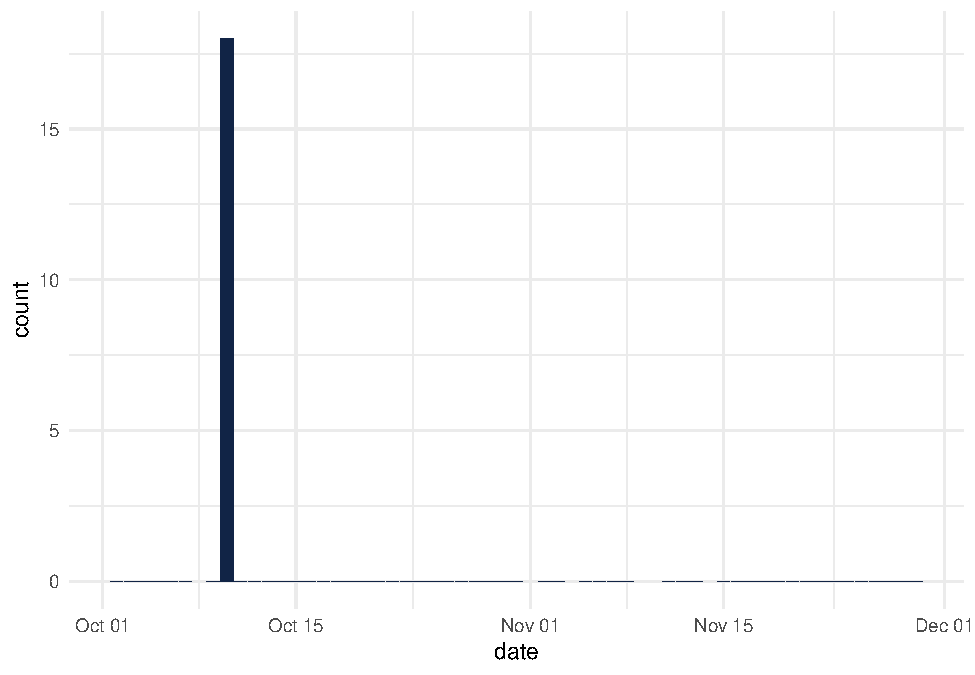
\includegraphics{project1_files/figure-latex/unnamed-chunk-6-1.pdf}

the day that has the maximun number of steps is 2012-10-10

\hypertarget{fourd-question}{%
\section{fourd question}\label{fourd-question}}

\begin{Shaded}
\begin{Highlighting}[]
\NormalTok{steps\_na }\OtherTok{\textless{}{-}} \FunctionTok{sum}\NormalTok{(}\FunctionTok{is.na}\NormalTok{(data}\SpecialCharTok{$}\NormalTok{steps))}
\NormalTok{date\_na }\OtherTok{\textless{}{-}} \FunctionTok{sum}\NormalTok{(}\FunctionTok{is.na}\NormalTok{(data}\SpecialCharTok{$}\NormalTok{date))}
\NormalTok{interval\_na }\OtherTok{\textless{}{-}} \FunctionTok{sum}\NormalTok{(}\FunctionTok{is.na}\NormalTok{(data}\SpecialCharTok{$}\NormalTok{interval))}
\end{Highlighting}
\end{Shaded}

\begin{enumerate}
\def\labelenumi{\arabic{enumi}.}
\item
  In this dataset i could found that we has 2304 NA values at the steps
  column, 0 NA values at the date column and 0 NA values at the interval
  column
\item
  fill de Na values in the dataset
\end{enumerate}

\begin{Shaded}
\begin{Highlighting}[]
\NormalTok{fill\_data }\OtherTok{\textless{}{-}} \FunctionTok{merge}\NormalTok{(data, data1, }\AttributeTok{by =} \StringTok{"date"}\NormalTok{)}

\NormalTok{fill\_data}\SpecialCharTok{$}\NormalTok{steps\_adj }\OtherTok{\textless{}{-}} \FunctionTok{ifelse}\NormalTok{(}\FunctionTok{is.na}\NormalTok{(fill\_data}\SpecialCharTok{$}\NormalTok{steps), fill\_data}\SpecialCharTok{$}\NormalTok{mean, fill\_data}\SpecialCharTok{$}\NormalTok{steps)}
        

\NormalTok{fill\_data }\SpecialCharTok{\%\textgreater{}\%}
 \FunctionTok{ggplot}\NormalTok{() }\SpecialCharTok{+}
  \FunctionTok{aes}\NormalTok{(}\AttributeTok{x =}\NormalTok{ date, }\AttributeTok{weight =}\NormalTok{ steps) }\SpecialCharTok{+}
  \FunctionTok{geom\_bar}\NormalTok{(}\AttributeTok{fill =} \StringTok{"\#112446"}\NormalTok{) }\SpecialCharTok{+}
  \FunctionTok{theme\_minimal}\NormalTok{()}
\end{Highlighting}
\end{Shaded}

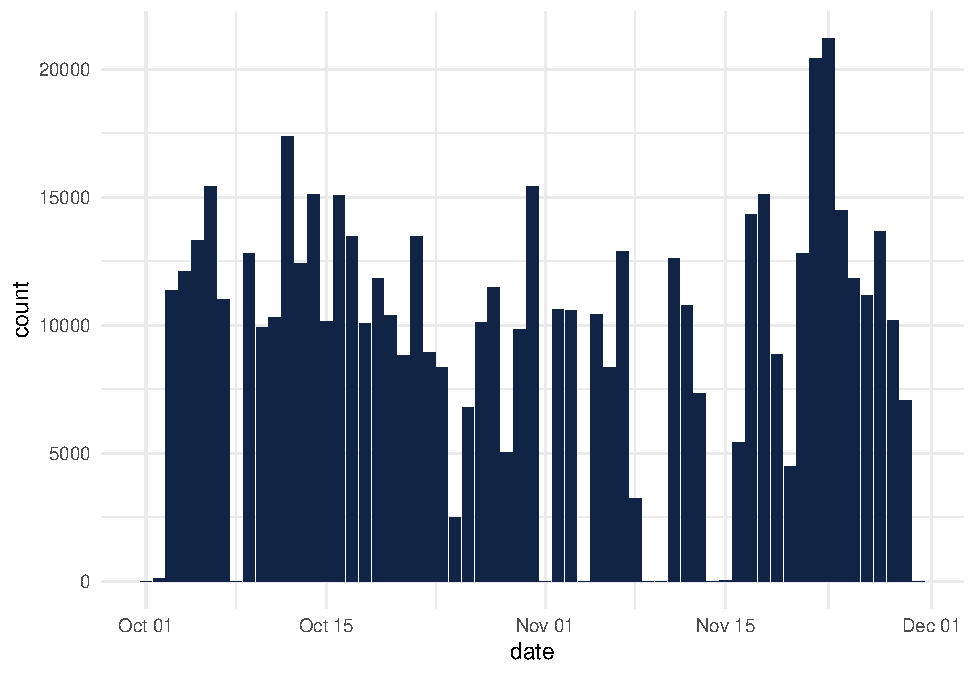
\includegraphics{project1_files/figure-latex/unnamed-chunk-8-1.pdf}

when all the values filled we can see that the values for the mean and
median per day looks like

\begin{Shaded}
\begin{Highlighting}[]
\NormalTok{data2 }\OtherTok{\textless{}{-}}\NormalTok{ fill\_data }\SpecialCharTok{\%\textgreater{}\%} 
        \FunctionTok{select}\NormalTok{(date, steps) }\SpecialCharTok{\%\textgreater{}\%} 
        \FunctionTok{group\_by}\NormalTok{(date) }\SpecialCharTok{\%\textgreater{}\%} 
        \FunctionTok{summarise}\NormalTok{(}\AttributeTok{median =} \FunctionTok{median}\NormalTok{(steps), }\AttributeTok{mean =} \FunctionTok{mean}\NormalTok{(steps))}

\FunctionTok{kbl}\NormalTok{(data2) }\SpecialCharTok{\%\textgreater{}\%} 
        \FunctionTok{kable\_styling}\NormalTok{()}
\end{Highlighting}
\end{Shaded}

\begin{table}
\centering
\begin{tabular}[t]{l|r|r}
\hline
date & median & mean\\
\hline
2012-10-01 & NA & NA\\
\hline
2012-10-02 & 0 & 0.4375000\\
\hline
2012-10-03 & 0 & 39.4166667\\
\hline
2012-10-04 & 0 & 42.0694444\\
\hline
2012-10-05 & 0 & 46.1597222\\
\hline
2012-10-06 & 0 & 53.5416667\\
\hline
2012-10-07 & 0 & 38.2465278\\
\hline
2012-10-08 & NA & NA\\
\hline
2012-10-09 & 0 & 44.4826389\\
\hline
2012-10-10 & 0 & 34.3750000\\
\hline
2012-10-11 & 0 & 35.7777778\\
\hline
2012-10-12 & 0 & 60.3541667\\
\hline
2012-10-13 & 0 & 43.1458333\\
\hline
2012-10-14 & 0 & 52.4236111\\
\hline
2012-10-15 & 0 & 35.2048611\\
\hline
2012-10-16 & 0 & 52.3750000\\
\hline
2012-10-17 & 0 & 46.7083333\\
\hline
2012-10-18 & 0 & 34.9166667\\
\hline
2012-10-19 & 0 & 41.0729167\\
\hline
2012-10-20 & 0 & 36.0937500\\
\hline
2012-10-21 & 0 & 30.6284722\\
\hline
2012-10-22 & 0 & 46.7361111\\
\hline
2012-10-23 & 0 & 30.9652778\\
\hline
2012-10-24 & 0 & 29.0104167\\
\hline
2012-10-25 & 0 & 8.6527778\\
\hline
2012-10-26 & 0 & 23.5347222\\
\hline
2012-10-27 & 0 & 35.1354167\\
\hline
2012-10-28 & 0 & 39.7847222\\
\hline
2012-10-29 & 0 & 17.4236111\\
\hline
2012-10-30 & 0 & 34.0937500\\
\hline
2012-10-31 & 0 & 53.5208333\\
\hline
2012-11-01 & NA & NA\\
\hline
2012-11-02 & 0 & 36.8055556\\
\hline
2012-11-03 & 0 & 36.7048611\\
\hline
2012-11-04 & NA & NA\\
\hline
2012-11-05 & 0 & 36.2465278\\
\hline
2012-11-06 & 0 & 28.9375000\\
\hline
2012-11-07 & 0 & 44.7326389\\
\hline
2012-11-08 & 0 & 11.1770833\\
\hline
2012-11-09 & NA & NA\\
\hline
2012-11-10 & NA & NA\\
\hline
2012-11-11 & 0 & 43.7777778\\
\hline
2012-11-12 & 0 & 37.3784722\\
\hline
2012-11-13 & 0 & 25.4722222\\
\hline
2012-11-14 & NA & NA\\
\hline
2012-11-15 & 0 & 0.1423611\\
\hline
2012-11-16 & 0 & 18.8923611\\
\hline
2012-11-17 & 0 & 49.7881944\\
\hline
2012-11-18 & 0 & 52.4652778\\
\hline
2012-11-19 & 0 & 30.6979167\\
\hline
2012-11-20 & 0 & 15.5277778\\
\hline
2012-11-21 & 0 & 44.3993056\\
\hline
2012-11-22 & 0 & 70.9270833\\
\hline
2012-11-23 & 0 & 73.5902778\\
\hline
2012-11-24 & 0 & 50.2708333\\
\hline
2012-11-25 & 0 & 41.0902778\\
\hline
2012-11-26 & 0 & 38.7569444\\
\hline
2012-11-27 & 0 & 47.3819444\\
\hline
2012-11-28 & 0 & 35.3576389\\
\hline
2012-11-29 & 0 & 24.4687500\\
\hline
2012-11-30 & NA & NA\\
\hline
\end{tabular}
\end{table}

\hypertarget{fifth-question}{%
\section{fifth question}\label{fifth-question}}

\begin{Shaded}
\begin{Highlighting}[]
\NormalTok{fill\_data}\SpecialCharTok{$}\NormalTok{weekday }\OtherTok{\textless{}{-}} \FunctionTok{weekdays}\NormalTok{(fill\_data}\SpecialCharTok{$}\NormalTok{date)}

\NormalTok{fill\_data}\SpecialCharTok{$}\NormalTok{weekday1 }\OtherTok{\textless{}{-}} \FunctionTok{ifelse}\NormalTok{(fill\_data}\SpecialCharTok{$}\NormalTok{weekday }\SpecialCharTok{==} \StringTok{"Saturday"} \SpecialCharTok{|}\NormalTok{ fill\_data}\SpecialCharTok{$}\NormalTok{weekday }\SpecialCharTok{==} \StringTok{"Sunday"}\NormalTok{, }\StringTok{"Weekend"}\NormalTok{, }\StringTok{"Weekday"}\NormalTok{)}

\NormalTok{fill\_data1 }\OtherTok{\textless{}{-}}\NormalTok{ fill\_data }\SpecialCharTok{\%\textgreater{}\%}
        \FunctionTok{select}\NormalTok{(steps\_adj, interval, weekday1) }\SpecialCharTok{\%\textgreater{}\%} 
        \FunctionTok{group\_by}\NormalTok{(interval, weekday1) }\SpecialCharTok{\%\textgreater{}\%} 
        \FunctionTok{summarise}\NormalTok{(}\FunctionTok{mean}\NormalTok{(steps\_adj))}
\end{Highlighting}
\end{Shaded}

\begin{verbatim}
## `summarise()` has grouped output by 'interval'. You can override using the
## `.groups` argument.
\end{verbatim}

\begin{Shaded}
\begin{Highlighting}[]
\FunctionTok{ggplot}\NormalTok{(fill\_data1) }\SpecialCharTok{+}
  \FunctionTok{aes}\NormalTok{(}\AttributeTok{x =}\NormalTok{ interval, }\AttributeTok{y =} \StringTok{\textasciigrave{}}\AttributeTok{mean(steps\_adj)}\StringTok{\textasciigrave{}}\NormalTok{) }\SpecialCharTok{+}
  \FunctionTok{geom\_step}\NormalTok{(}\AttributeTok{colour =} \StringTok{"\#112446"}\NormalTok{) }\SpecialCharTok{+}
  \FunctionTok{theme\_minimal}\NormalTok{() }\SpecialCharTok{+}
  \FunctionTok{facet\_wrap}\NormalTok{(}\FunctionTok{vars}\NormalTok{(weekday1))}
\end{Highlighting}
\end{Shaded}

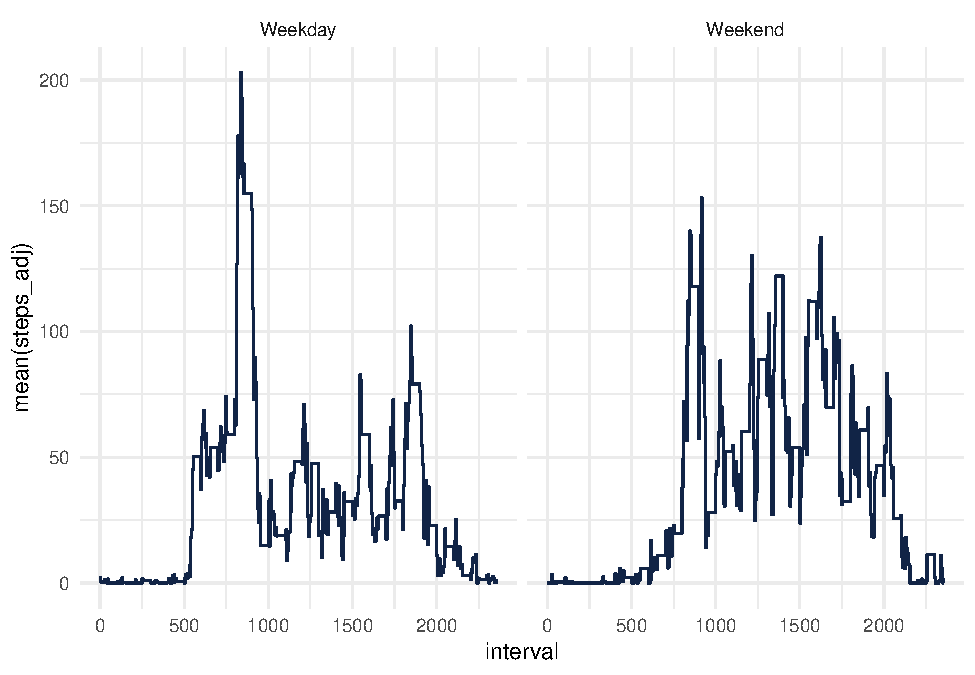
\includegraphics{project1_files/figure-latex/unnamed-chunk-10-1.pdf}

\end{document}
